\documentclass[a4paper]{article}

%% Language and font encodings
\usepackage[english]{babel}
\usepackage[utf8x]{inputenc}
\usepackage[urw-garamond]{mathdesign}
\usepackage[T1]{fontenc}
\usepackage{mathptmx}
\usepackage[12pt]{moresize}
%% \usepackage{ebgaramond,newtxmath,ebgaramond-maths}

%% Sets page size and margins
\usepackage[a4paper,top=1in,bottom=1in,left=1in,right=1in,marginparwidth=1.75cm]{geometry}

\usepackage{setspace}
\onehalfspacing


%% Useful packages
\usepackage{amsmath}
\usepackage{graphicx}
\usepackage[colorinlistoftodos]{todonotes}
\usepackage[colorlinks=true, allcolors=blue]{hyperref}
\usepackage{natbib}
\setlength{\bibsep}{0pt plus 0.3ex}
\usepackage{algorithm}
\usepackage{tikz}
\usepackage[noend]{algpseudocode}
\usepackage{float}


\newcommand{\norm}[1]{\left\lVert#1\right\rVert}

\title{House Price Prediction with Machine Learning}
\author{Keping Wang}

\begin{document}
\maketitle

\begin{abstract}
This paper introduces various machine learning methods for house prediction. Experiments are conducted to choose the best model for this task, and support vector regression is the winner.
\end{abstract}

\section{Introduction}
House Price Prediction, or Hedonic Regression, is an important topic in real estate economics. Once we can accurately predict the house price given various features of the house, the prediction model can be applied to other economics tasks such index constructing, house value assessment, and analyzing demand for various housing characteristics. Yet economists are more familiar with causal inference than prediction. At the same time, the machine learning field, where some statisticians and computer scientists work on, is dedicated at making predictions. So I decide to write this paper to introduce the machine learning methods for economists interested at house price prediction. The techniques introduced here can be applied to other prediction tasks as well. 

This paper has two main themes:
\begin{enumerate}
  \item Introducing the machine learning methods and explaining why they are better at making predictions than simple linear regressions.
  \item Exploring by experiments the best machine learning method for house price prediction.
\end{enumerate}

The paper is organized as follows: 1) this brief introduction, 2) section 2 briefly reviews the economics literature of house price prediction with machine learning methods; 3) section 3 introduces the supervised learning framework, with emphasis on gradient descent, non-linearity, prediction VS causality, regularization, and cross-validation; 4) section 4 shows the four supervised learning models I'm going to compare, linear regression with L2 regularization, Lasso regression, support vector regression, and random forest regression; 5) section 5 compares the prediction results of the various models; 6) section 6 introduces an unsupervised learning technique called principal component analysis; 7) section 7 compares different feature selection methods; and finally 8) section 8 is the conclusion.

\section{Economics Literature}
Many researchers have shown that certain machine learning techniques are more powerful at house price prediction than the traditional Ordinary Least Squares (OLS) model. \cite{yoo2012variable} uses a Random Forest model for variable selection during hedonic regression and shows that it achieves an $R^2$ of 0.97, while an OLS of similar configuration only got $R^2$ of 0.76.
\cite{Selim20092843} compares OLS and Artificial Neural Networks (ANN)\footnote{I also tried ANN, but it performs worse than other methods. So I choose not to introduce it in this paper.} using the house price data of Turkey and finds out that the Root Mean Squared Error (RMSE, the smaller, the better) of OLS and ANN are 1.57 and 0.66 respectively.

Some researchers don't exploit the machine learning methods for hedonic regression, but trying to improve the prediction accuracy by manually engineering features. For example, during the attempt of wine price prediction, \cite{costanigro2007segmenting} finds that fitting different kinds of wines differently greatly improves the model accuracy. Although machine learning nowadays still rely on human feature engineering for top performance, the kind of feature engineering in their paper could be automatically accomplished by a machine learning model.

Computer scientists and statisticians study machine learning for the single purpose of making predictions. It is understandable that machine learning methods are better at fitting values than the traditional econometric approaches. Just as \cite{AtheyQuora} said on Quora\footnote{\url{https://www.quora.com/How-will-machine-learning-impact-economics?redirected_qid=6706789}}, machine learning will have enormous impact on economics. Her work is concentrated on applying machine learning to causal inference, where some tweaks of the machine learning models have to be made. However, for tasks like hedonic house price prediction, the only goal is prediction accuracy, then many off-the-shelf machine learning methods would be sufficient.

\section{Supervised Learning Framework}
In this section I will briefly introduce the machine learning methods that I will try to apply to the hedonic house price regression problem. All these methods fall into the category of supervised learning, where the true data $y$ is provided, and the model is trained to take input $X$ and generate an output that is as similar to $y$ as possible. 

Under supervised learning, there are two general categories of problems, classification and regression. The difference is that the truth variables $y$ in classification task only take a limited number of discrete values, while the $y$ in prediction take continuous values. Hedonic house prediction fits exactly into the supervised regression task.

From now on, let's take an OLS model and I'll use it to illustrate the machine learning techniques. Here is the OLS model:
\begin{equation}
\hat{y} = f(x) = w\cdot x + b,
\end{equation}
where $x$ is a vector of features (like number of bedrooms, floor size, etc...), $w$ is a vector denoting the weight of these features, and $b$ is a bias term to "shift" the predicted values.

A supervised learning task is to choose the $w$ and $b$ variables so that $y$ and $yhat$ is as similar as possible. We need an exact measure of how similar $y$ and $yhat$ are, and we call that the loss function. For regression tasks, it usually takes the following form, Mean Squared Error (MSE):
\begin{equation}
loss = \frac{1}{n}\sum_i^n \left( y_i - f(x_i) \right)^2.
\end{equation}

Then the our OLS task becomes choosing $w$ and $b$ variables so as to minimize the loss. There are three possible approaches for this optimization task:
\begin{enumerate}
 \item Randomly try all $w$ and $b$ from the range of all real numbers and keep the variables that lead to the smallest loss. This is stupid and I am just kidding.
 \item Solve the quadratic optimization problem mathematically and calculate the value of $w$ and $b$ from the math solution. In OLS, we would have $w = (X′X)^{-1}X′Y$. The solution looks neat, but there are problems with this approach:
 \begin{enumerate}
  \item Not general enough. For each different kind of model $\hat{y} = f(x)$, the math has to be redone to calculate the best weights. The calculation is simple for OLS, but for more complex models, it becomes hardly possible to derive a straight math solution. For example, think of a non-linear regression model: $f(x) = w_2 \cdot \frac{1}{1+ e^{-w_1\cdot x}}$, where $x$ is of dimension $k$, $w_1$ is of dimension $k\times h$, and $w_2$ is of dimension $h$.
  \item Computationally very expensive both in terms of time and memory \citep{CookInvMat}. It takes $O(n^3)$ time and $O(n^2)$ memory. When $n$ becomes as large as one million, it would require terabytes of memory.
 \end{enumerate}
\item In the machine learning area, people use a technique called gradient descent to find the optimal weight. The only requirement for gradient descent is that the loss function is differentiable. The loss function could be formulated as $loss(y,X,w)$ where $y$ and $X$ are input values and are treated as constant during optimization, while $w$ denotes all the weight variables (including the bias terms). Gradient of the loss with respect to the weight is:
\begin{equation}
 \nabla_w loss(y,X,w),
\end{equation}
and the gradient descent algorithm is the following:

\begin{algorithm}
\caption{Gradient Descent}\label{euclid}
\begin{algorithmic}[1]
\State Choose hyperparameter learning rate $\alpha$ 
\State Initialize $w$ with some initial value
\Repeat
\State $w = w - \alpha \nabla_w loss(y,X,w)$
\Until{in an iteration, the change of the loss is small enough}
\end{algorithmic}
\end{algorithm}

Gradient descent is a general algorithm, in that as long as the loss function is differentiable (don't even need to be globally differentiable), the gradient of weight variables $w$ could be calculated using chain rules. And for constrained optimization problems, they can first be converted to unconstrained optimization problems using Lagrange multiplier method, and then solved by applying gradient descent.
\end{enumerate}

To summarize, our supervised learning regression task has become: picking a model $f(x;w)$, with $w$ as parameters, and train the model to minimize loss using gradient descent. The researcher's task is more or less mainly about picking the right model $f(x;w)$.

\subsection{Beyond Linearity}
One advantage of this supervised learning framework over traditional linear regression is that the model $f(x;w)$ can be flexible and incorporates all kinds of non-linearity. Because we have the magic tool of gradient descent, our model $f(x;w)$ could take various forms and the calculation will be the same. 

Economists have been playing a lot with various flavors of linear regression and inference of estimation error. Linear regression is good because its simplicity allows economists to easily derive estimation errors for the weights, understand the model, and convey the understanding to the general audience. 

Most non-linear models cannot really be easily summarized in one or two sentences to convey the finding, but they can involve complicated logics and are well-suited for making predictions. Non-linearity really brings magic to prediction. Think of AlphaGo and self-driving cars, they are all enabled by various kinds of non-linearity in the machine learning model.

Let me use house price prediction as an example to show how non-linearity makes the prediction model more powerful. Imagine there to be a feature (one dimension of the input $X$), describing whether there is a swimming pool. If you include the swimming pool feature into a simple linear regression, you find that it increases house price by $20000$ dollars on average. However, likely a more accurate estimation is that for great neighborhoods the a swimming pool adds the price by $40000$, while for not-so-good neighborhoods it only adds the prices by $10000$. 

Then the classic econometric way of handling this is to include the interaction term of neighborhood quality and swimming pool $(neighborhood \times pool)$. That is acceptable when we have a very limited number of variables. But when we are predicting using many variables, the interactions between variables are usually to complicated to specify manually.

Using non-linear models, we could handle complex interactions automatically. In this example, the model specification could be $f = sign(w_1 neighborhood + b_1) \cdot w_2pool$, which can serve the same functionality as the interaction term. We do still have to manually choose from a range of supervised learning models, just as we have to pick interaction terms manually. But some supervised learning models have the power to allow enormously different kinds of interactions between variables, and they can be trained very easily, then only those interactions that do help with the prediction will remain with a large enough weight (coefficient).

\subsection{Feature Selection}
Feature selection, or variable selection is very important for a prediction model. Sometimes the original data contains lots of duplicate or useless features, and including these features will consume some degrees of freedom\footnote{Degree of freedom only applies to linear regression. But for non-linear models there are similar mechanisms where including useless features make the model worse.}. If we had an unlimited number of observations, then for some flexible models, more features will strictly improve performance. With a limited number of observations, we would still want to do feature selection. However, feature selection has to be done automatically, instead of manually, since there could be a huge amount of features and we are trying to find a general approach for house price prediction.

\subsection{Prediction instead of Causality}
Another difference between the supervised learning method and the econometrics method is that in supervised learning, prediction is the only goal and it doesn't care anything about causal inference. \cite{AtheyQuora} has been working on modifying machine learning methods for causal inference, but that is not the focus of this paper.

Prediction doesn't care about omitted variables. For prediction, the more variables, the better, but we can hardly exhaust all the variables. Also prediction here only provides information about expected values, but not about confidence.

\subsection{Regularization and Cross-Validation}
To show how accurate is our model for prediction, we cannot only see the $R^2$ of the fitted values for our training data set. With a complex model specification, it is always possible to perfectly fit a very small dataset, but then this model won't be able to generalize well to unseen data.

So the model needs to be evaluated using unseen data. This is called test set. At the very beginning I randomly choose part of the data as the test data, keep them away from the training process, and only use the test data finally for evaluating accuracy.

A good prediction model, should on the one hand be complex enough to incorporate the interactions of variables, but on the other hand be limited so as to generalize well to unseen data. Generally speaking, the methods used to limit the "power" of the model is called regularization.

One regularization method I'm going to use here is the explicit L2 regularization. That is, for each weight (coefficient) $w$, a regularization term $reg * w^2$ is added to the total loss of the model, where $reg$ is a hyperparameter to be chosen before training. This regularization means that there is a cost for using each additional weight, i.e. it is better to fit the model with as fewer weight nodes.

Another technique for finding better model is cross-validation. For each category of models, there are hyperparameters to determine before training, for example, what variables to include. These hyperparameters has to be decided on another separate dataset called validation data. The validation data is usually held out apart from the original training data, and is also separate from the test data. 

The last technique I'll be using to make the model better at generalization is called stochastic gradient descent (SGD). SGD still iterates to optimize the weights but in each iteration it uses a random mini-batch (could be 50 samples) of training data, instead of the whole training data. \cite{zhang2016understanding} has shown that SGD is implicitly regularizing the solution. 

In the next section I'll briefly introduce the supervised learning models that I'll use for house price prediction: support vector regression, random forest regression, and neural networks.

\section{Supervised Learning Models}

\subsection{Linear Regression with L2 Regularization}
In linear regression with L2 regularization, our model for prediction is still
\begin{equation}
  f(X) = XW + b,
\end{equation}
but our loss function to minimize becomes:
\begin{equation}
  loss = \norm{y - (XW+b)}^2_2 + \lambda \norm{W}^2_2,
\end{equation}
where $\norm{a}_2$ means the L2 norm of $a$, that is $\norm{a}_2 = \sqrt{\sum_i a_i^2}$.

Here $\norm{W}^2_2$ is the regularization term, which will try to make the model parameters close to zeros. The term $\norm{y - (XW+b)}_2$ term on the left will try to make the model fit as much as it could on the training data. Thus the fitting term and regularization term work together to make give the model good performance on the test set. $\lambda > 0$ denotes the strength of regularization, and it is a hyperparameter of the model, to be determined using the validation set. 

\subsection{Lasso Regression}
Lasso (least absolute shrinkage and selection operator) regression also uses the same linear fitting term, but uses L1 norm for regularization and performs automatic feature selection. The loss function is:
\begin{equation}
  loss = \norm{y - (XW+b)}^2_2  + \lambda \norm{W}_1,
\end{equation}
where $\norm{a}_1$ means the L1 norm of $a$, that is $\norm{a}_1 = \sum_i |a_i|$.

It can be helpful to think of the two problems in constrained form \citep{cmuLasso}:
\begin{align}
  \min \norm{y - (XW+b)}^2_2  & \quad \text{subject to } \norm{W}^2_2 \leq t \\
  \min \norm{y - (XW+b)}^2_2  & \quad \text{subject to } \norm{W}_1 \leq t
\end{align}
Now $t$ is the hyperparameter. For any $\lambda$ and corresponding solution in the previous formulation, there is a value of $t$ such that the above constrained form has the same solution.

\begin{figure}[H]
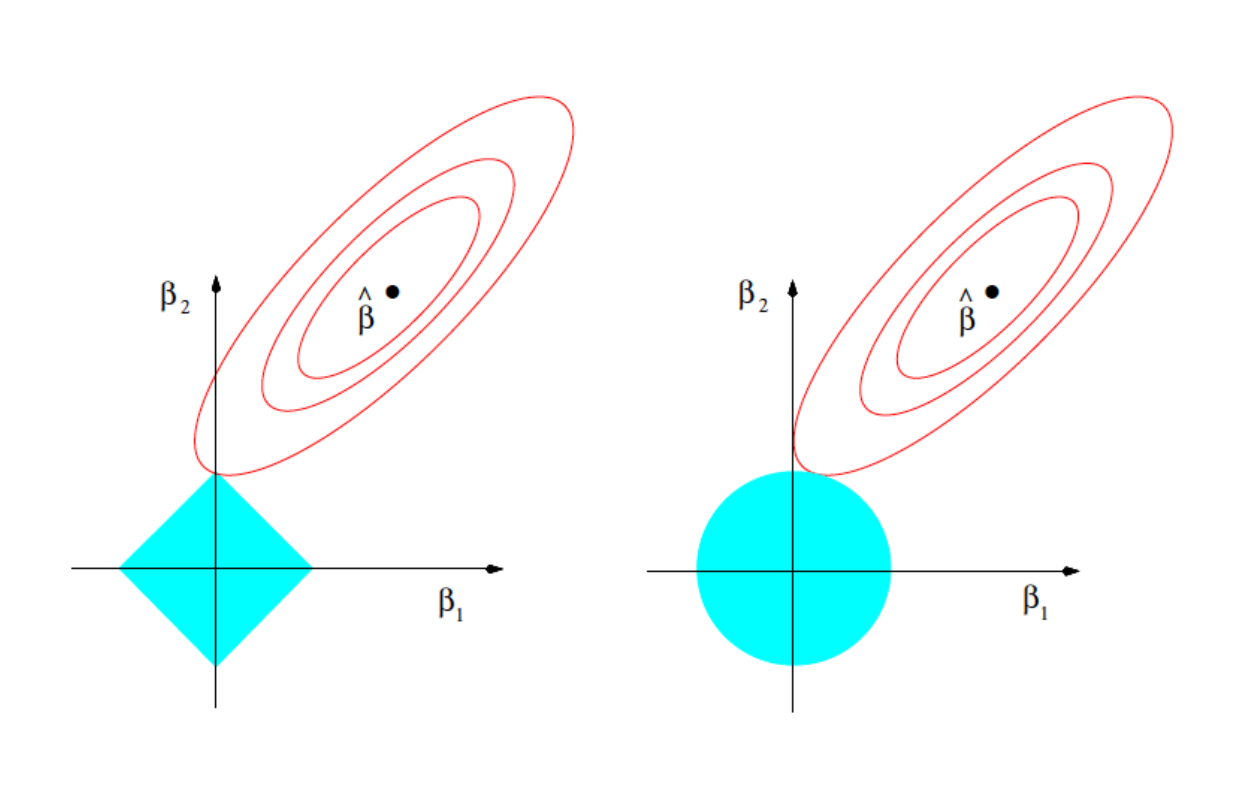
\includegraphics[width=\textwidth]{lasso_ridge.png}
\caption{Linear Regression: L1 vs L2 regularization}
\end{figure}

The graph\footnote{Picture taken from \cite{cmuLasso}} illustrates the difference between L1 norm and L2 norm weight regularization. The figure shows the case where the weight $W$ contains only two dimensions, $\beta_1$, and $\beta_2$. $\hat{\beta}$ in the graph denotes the weight $W$ that best fits the linear prediction part of the model. The light blue shapes (square or circle) denotes the constraints applied by the regularization term, and the size of the constraint area will change with regularization strength $\lambda$.

The main difference here is that L1 regularization allows weight parameters to be exactly zero, which means the solution falls on some corner cases, which for L2 regularization, the weight can hardly be exactly zero. 

Because L1 regularization renders zero weights for some variables, Lasso regression utilizes this fact to do feature selection. There are some specific approaches for how features are selected, but the one I use here goes as follows:
\begin{algorithm}
\caption{Feature Selection for Lasso}
\begin{algorithmic}[1]
\State Initialize $K$ to be the set of all features.
\Repeat
\State Run Lasso with feature set $K$, get feature weights.
\State $K = $ features in $K$ with non-zero weights.
\Until{all features in $K$ has non-zero weights.}
\end{algorithmic}
\end{algorithm}

By applying feature selection, lasso increase the robustness of the model by removing the random influences of useless features.

Linear regression with regularization could be viewed as either 1) unconstrained  optimization, which could be solved in general by gradient descent, or 2) constrained quadratic (and convex) optimization, which could be solved by quadratic programming.

\subsection{Support Vector Regression}

Support vector regression \citep{basak2007support} has the following optimization objective:

\begin{align}
\text{minimize} \quad & \frac{1}{2} \norm{W} + C \sum_{i=1}^{n} (\xi_i + \xi_i^*) \\
\text{subject to} \quad & - \epsilon  -\xi_i^* \leq y_i -  W \cdot x_i - b \leq \epsilon + \xi_i \\
& \xi_i, \xi_i^2 \geq 0
\end{align}

This seems intimidating, but let me introduce the general ideas with the help of the graph\footnote{Graph taken from \cite{basak2007support}}.

\begin{figure}[H]
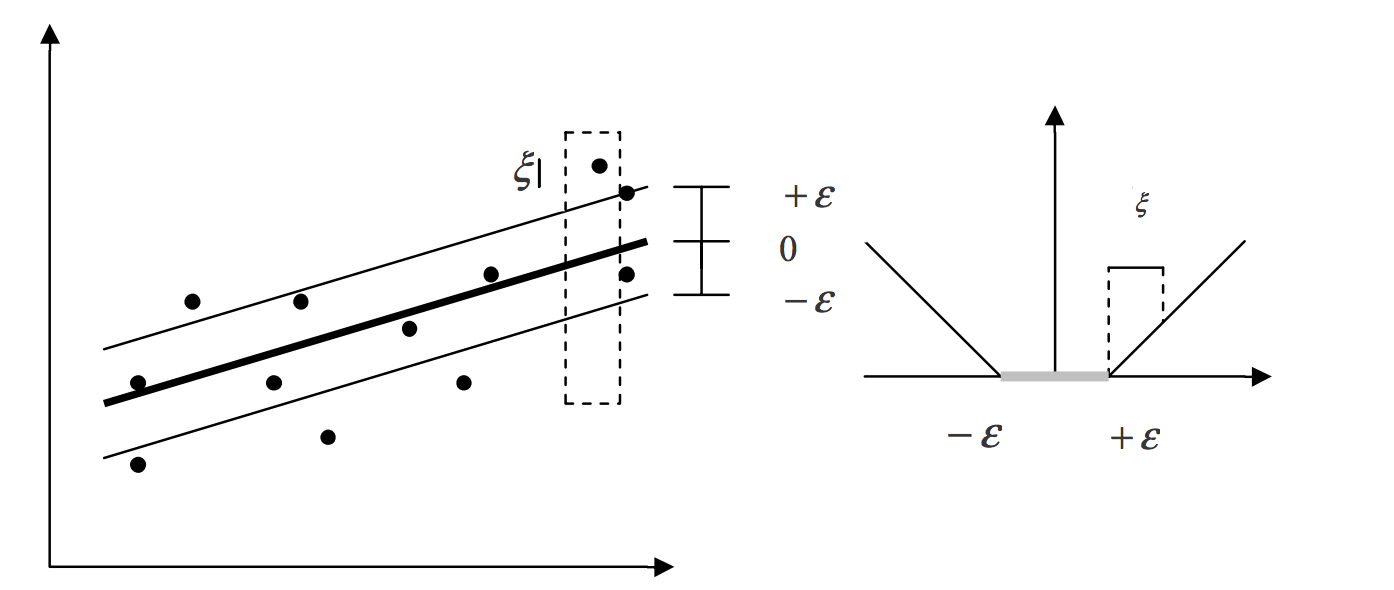
\includegraphics[width=\textwidth]{svr.png}
\caption{Soft Margin Linear SVR}
\end{figure}

For now, the prediction term is still $WX + b$. In the constraints of the objective, we can see that the error of prediction is actually constrained to be within the interval $(-\epsilon -\xi^*, \epsilon + \xi)$. The $\epsilon$ part is the hard margin constraint, and the $\xi$ part is the soft margin constraint. $\epsilon$ is a hyperparameter of the model, rather than a parameter to be learned. 

If we ignore all $\xi$ terms, the model becomes: you must fit the data so that all fitting errors fall within $(-\epsilon, \epsilon)$. When the hard condition is met, try to minimize the L2 norm of weight. If the data cannot be fitted with margin $\epsilon$, then the margin SVR problem has no solution. 

Adding $\xi$ terms softens the margin and makes sure there is always a feasible solution. The data point that falls out of $(-\epsilon, \epsilon)$ thus adds penalty to the objective function. $C > 0$ is the strength of penalty for data points outside of hard margin. 

The main characteristic of Support Vector Regression is that only data points within the margin $(-\epsilon, \epsilon)$ are involved in calculating the weight (especially when $C$ is close to $zero$), and these data points are called support vectors. Therefore the model is very resilient to outliers. The power of SVR lies more in its dual form:

\begin{align}
  \text{maximize} \quad & -\frac{1}{2} \sum_{i,j} (\alpha_i - \alpha_i^*) (\alpha_j - \alpha_j^*) \langle x_i, x_j \rangle - \epsilon \sum_i (\alpha_i + \alpha^*_i) + \sum_i y_i (\alpha_i - \alpha_i^*) \\
  \text{subject to} \quad & \sum_i (\alpha_i - \alpha_i^*) = 0 \text{ and } \alpha_i, \alpha_i^* \in [ 0, C ] 
\end{align}

The relationship between the solution of the primal problem and the dual problem is:
\begin{equation}
  W = \sum_i (\alpha_i - \alpha_i^*) x_i \quad \text{ and therefor, } f(x) = \sum_i(\alpha_i - \alpha_i^*) \langle x_i, x \rangle + b
\end{equation}
This is called support vector expansion, i.e., $W$ can be completely described as a linear combination of the training patterns $x_i$. Even for evaluating $f(x)$, we don't need to compute $W$ explicitly. 

This dual problem can be solved with 1) quadratic programming, 2) Lagrange multipliers and gradient descent, or 3) some faster specific algorithms.

The advantage of the dual that we can than apply kernel trick. To understand kernel trick, let's pause and think about feature space transformation. If we want to use three features to fit a linear model, it would be like $f(x) = w_1x_1 + w_2x_2 + w_3x_3 + b$. If we want to allow for more flexibility, we probably would add square terms of features to the model $f(x) = w_1x_1 + w_2x_2 + w_3x_3 + w_4 x_1^2 + w_5 x_2^2 + w_6 x_3^3$. Then we probably want to add interaction terms too: $x_1x_2$, $x_1x_3$, and $x_2x_3$. Then it starts to make us economists uncomfortable when we are dealing with many more variables and want to manually add higher order terms and higher order interaction terms. This kind of feature space transformation can be done automatically with kernel trick.

If we have two data points $x^{(1)}$ and $x^{(2)}$. We can have the following equation \citep{konstantin}:
\begin{align}
k(x^{(1)}, x^{(2)}) = & (x^{(1)} \cdot x^{(2)})^2 = (\sum_i x_i^{(1) x_i^{(2)}})^2 = \sum_{i,j} x^{(1)}_i x^{(1)}_j x^{(2)}_i x^{(2)}_j \\
= & (x^{(1)}_1 x^{(1)}_2 + x^{(1)}_1 x^{(1)}_3 + x^{(1)}_2 x^{(1)}_3 ) \cdot (x^{(2)}_1 x^{(2)}_2 + x^{(2)}_1 x^{(2)}_3 + x^{(2)}_2 x^{(2)}_3 )
\end{align}
so the squared inner products of two data points can be used to represent the inner products all their interaction terms. This $k(x^{(1)}, x^{(2)})$ is called a kernel function, which can represent a feature space transformation by some calculations between two data points. Adding kernel functions will concatenate the feature space they represent. $k(x^{(1)}, x^{(2)}) = x^{(1)} \cdot x^{(2)} + (x^{(1)} \cdot x^{(2)})^2 $ represents the inner product of two data points in the following feature space:
\begin{equation}
  \left[x_1, x_2, x_3, x_1x_2, x_1x_3, x_2x_3\right].
\end{equation}

By plugging different forms of kernel function $k(x_i, x_j)$\footnote{ The notation $k(x^{(1)}, x^{(2)})$ and $k(x_i, x_j)$ both represent the kernel function, only I write the parameters in different forms. Later also $k(x, y)$. } back into our dual SVR problem to replace $\langle x_i, x_j \rangle$, we can fit the model with different kinds of feature space transformation. Sometimes the feature space is very huge because of all the higher order terms and interaction terms, but dual SVR with kernel trick could solve the problem easily. 

A kernel function often used is the RBF (Gaussian) kernel:
\begin{equation}
  k(x, y) = \exp \left( - \frac{\norm{x-y}^2}{2\sigma^2} \right) = \exp \left( - \gamma \norm{x-y}^2 \right),
\end{equation}
which represents a normalized polynomial infinite degree feature space transformation:
\begin{equation}
 \phi(x) = e^{-\gamma x^2} \left[ 1, \sqrt{\frac{2\gamma}{1!}} x, \sqrt{\frac{(2\gamma)^2}{2!}} x^2, \sqrt{\frac{(2\gamma)^3}{3!}} x^3, \cdots \right]
\end{equation}

To sum up, support vector machine can estimate weights ignoring far away data points and can use kernel functions to perform very complicated feature space transformation.

\subsection{Random Forest Regression}

Random Forest Regression\citep{liaw2002classification} is a method that's said to be a panacea for all data science problems. It differs from previously introduced models in two ways: 1) it is a tree-based model, which cannot be trained with the general gradient descent method; and 2) it is an ensemble of many models. Random Forest is an ensemble of multiple decision trees.

The following graph\footnote{The graph is made up for illustration, not representing real data.} illustrates a decision tree\footnote{Here it could be more precisely called a regression tree.} for house price prediction. The decision tree is trained by recursively split the data by a threshold of a feature until some ending condition is met. The numbers within parentheses are sample size. In the first step, a sample of size 100 is split to a 54 observations with living area $< 1800$ sqft, and 46 observations with living area $\geq 1800$ sqft. The feature used for splitting could be continuous, where a threshold value is taken, or categorical (or dummy), where true of false is used. The feature and its threshold used for splitting is chosen by some algorithm, so as to minimize the prediction loss (recursively at each step). 

At each step, the algorithm either goes on with splitting, or ends. The ending conditions could be things like maximum depth of a tree, or minimum size of subsample at a node. At a leaf node, we get a subsample meeting all previous conditions. For example, in the graph, we have 31 observations with living area $\geq 1800$ sqft and number of bedrooms at least 2, and the mean house sale price of these 31 observations is $\$140k$. 

This decision tree can then be used for prediction. If we have a house with living area 1900 sqft, 2 bedrooms, and one garage, this model will predict its house price to be $\$190k$.

\begin{figure}[H]
\centering
\begin{tikzpicture}[rectnode/.style={rectangle, draw=black!60, thick, minimum size=5mm},]
% nodes
\node (sample) at (0,0) {(100) sample};
\node[rectnode] (living_area) at (0, -1.5) {living area $\geq 1800$ sqft};
\node[rectnode] (num_bedroom_left) at (-2.5, -3) {\# bedrooms $\geq 2$};
\node[rectnode] (num_bedroom_right) at (2, -3) {\# bedrooms $\geq 3$};
\node (res1) at (-4, -4.5) {(23) $\$110k$};
\node (res2) at (-2, -4.5) {(31) $\$140k$};
\node[rectnode] (garage) at (1, -4.5) {has garage};
\node (res3) at (0, -6) {(3) $\$150k$};
\node (res4) at (2, -6) {(24) $\$190k$};
\node (res5) at (4, -4.5) {(19) $\$230k$};
% edges
\draw[->] (sample) -- (living_area);
\draw[->] (living_area) -- node[left] {False} (num_bedroom_left);
\draw[->] (living_area) -- node[right] {True} (num_bedroom_right);
\draw[->] (num_bedroom_left) -- node[left] {False} (res1);
\draw[->] (num_bedroom_left) -- node[right] {True} (res2);
\draw[->] (num_bedroom_right) -- node[left] {False} (garage);
\draw[->] (num_bedroom_right) -- node[right] {True} (res5);
\draw[->] (garage) -- node[left] {False} (res3);
\draw[->] (garage) -- node[right] {True} (res4);
\end{tikzpicture}
\caption{A Decision Tree predictor for house price}
\end{figure}

A decision tree is powerful in that it can provide the best possible fit for the training data if no ending condition is applied. In machine learning terms, we say this model has very low bias. The tree structure allows for a high level of non-linearity, and also does feature selection automatically in the sense that only features which result in the most fitted model will get involved in the tree building process. It can be viewed as automatically specifying many interaction terms, and only the ones that fit the data best.

However, a tree based model has very high variation, which means high generalization error. In the above graph, there are three data points that have living area $\geq 1800$ sqft, less than 3 bedrooms, and no garage.  They show that conditional on the living area $\geq 1800$ sqft and less than 3 bedrooms, the expected value of a garage is $\$40k$. It is possible that these 3 observations all happen to have particular poor conditions for some unobserved characteristics, and that the real value of a garage is only about $\$10k$. To reduce the model variance while maintaining the high fitting power of the decision tree, the random forest model use an ensemble of decision trees.

Model ensemble means grouping multiple models together for prediction. A random forest with 20 decision trees will get train these different trees from 20 different subsamples randomly drawn from the whole training dataset, and final predicted value is the mean of the predicted values of the 20 decision trees. 

A random forest model can have many hyperparameters, but a useful rule is to build each tree as deep as possible and to ensemble as many trees as possible. With this rule, we don't really need to tune any hyperparameters for a random forest. However, model performance does gets improved when the maximum number of features in trees is limited. Usually, thie maximum number of features is set to the square root of the total number of features.

To summarize, a random forest regression model is an ensemble of decision (regression) trees. It has low bias and low variance, and is very easy to tune.

\section{Experiments}
In this section, I'll introduce the data and preprocessing, evaluation metric of accuracy, and then show the results of different prediction models. All experiments are conducted in Python, with the help of the scikit-learn package \citep{scikit-learn}.

\subsection{Data and Preprocessing}
The data comes from \cite{de2011ames}. It describes the sale of individual residential property in Ames, Iowa from 2006 to 2010. The data set contains 2930 observations and a large number of explanatory variables (23 nominal, 23 ordinal, 14 discrete, and 20 continuous). Please refer to \cite{de2011ames} for a complete description of all variables. 

In my models, I treat discrete variables the same as continuous variables, encode ordinal variables with integer values starting from 0, and transform nominal variables using one-hot encoding. For continuous variables with skewed distributions, including the final sale price to predict, I make log transformations ($\phi(x) = \log(1+x)$) to make them closer to normal distribution. Finally, there are 271 features, meaning that the input matrix $X$ has 271 columns.

Here are the histograms of House Sale Price - the variable to predict, before and after log transformation.
\begin{figure}[H]
\centering
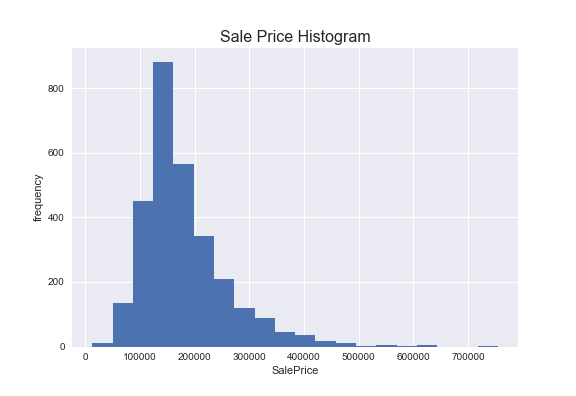
\includegraphics[width=0.4\textwidth]{sale_price_hist.png}
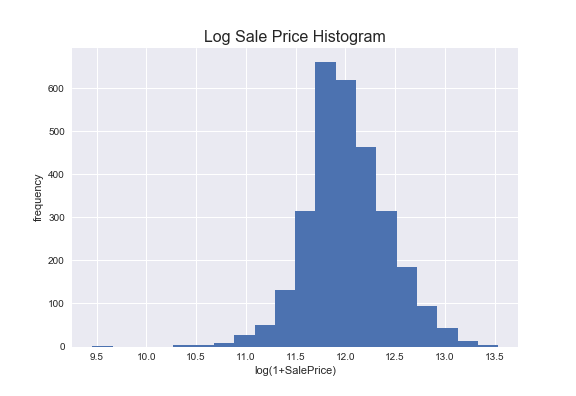
\includegraphics[width=0.4\textwidth]{log_sale_price_hist.png}
\caption{Sale Price distribution before and after log transformation.}
\end{figure}

I split the whole 2930 observations into a training set of 2200 observations, a validation set of 230 observations, and a test set of 500 observations. Here I don't bother to use k-fold cross validation, but only hold out the validation set. 

Before the training of the models, each input feature is standardized with mean and standard deviation from training set. Feature standardization allows gradient descent method and other training methods to work better. 

\subsection{Evaluation of Accuracy}

The loss we use here is the mean squared loss as mentioned above. And we use two measures of prediction accuracy, $R^2$ and RMSE (Root Mean Squared Error):
\begin{align}
& R^2 = 1 - \text{SSE}/ \text{SST}, \\
& RMSE = \sqrt{\text{SSE} / n}, \\
\text{where} \quad & \text{SSE} = \sum_i^n (y_i - f(x_i))^2, \\
 & \text{SST} = \sum_i^n (y_i - \bar{y}).
\end{align}
RMSE is more usually used in the machine learning literature, and it more directly measures the prediction error of a single data point. While $R^2$ is usually used in the econometrics literature to see how much total variation is explained by the fitted values. RMSE is a more direct measure of accuracy for prediction. Here I also include $R^2$ mostly for the convenience of the audience from an economics background.

\subsection{Prediction Results}
The models are trained on the training set. The hyperparameters are determined by running the model repeatedly with different hyperparameters, and choosing the hyperparameters that result in the best results in validation set. The tuned models are then evaluated using the test set, and these results show the final performance of the models.

Experiments are done with all four previously mentioned models: 1) linear regression with L2 loss, 2) Lasso regression, 3) support vector regression, and 4) random forest regression. For the first two models, the only hyperparameter is $\lambda$, the strength of regularization. SVR has two hyperparameters, $C$, error penalty strength, and $\epsilon$, specifying the tube within which no penalty is associated in the training loss function with points predicted within a distance epsilon from the actual value. Here I use an SVR with RBF kernel. For random forest, the only hyperparameter is the number of trees it ensembles. All these models have more hyperparameters, but I only choose to tune on the most important ones mentioned above.

\begin{table}[H]
\centering
\caption{\large Model Prediction Results}
\vspace{0.3cm}
\begin{tabular}{| r | p{2cm} | p{2cm} | p{2cm} |}
\hline
 & \multicolumn{3}{|c|}{Results: (RMSE, $R^2$)} \\
\hline
Model & Training & Validation & Test \\
\hline
Linear Regression without Regularization (OLS) & 0.0992, 0.940 & 1e7, -1e15 & 6e7, -2e16 \\
\hline
Linear Regression with L2 Regularization & 0.1143, 0.921 & 0.1162,0.922 & 0.1177, 0.918 \\
\hline
Lasso Regression & 0.1049, 0.933 & 0.1127, 0.927 & 0.1139, 0.923 \\
\hline
Support Vector Regression & 0.1199, 0.912 & 0.1041, 0.937 & 0.1133, 0.924 \\
\hline
Random Forest Regression & 0.0504, 0.985 & 0.1312, 0.900 & 0.1315, 0.898 \\
\hline
\end{tabular}
\end{table}

In the table, results are shown in (RMSE, $R^2$) pairs, and the test column is the final result. A model is good if it has a small RMSE and a large $R^2$. To note again, the training set has 2200 observations, the validation set has 230 observations, and the test set has 500 observations. Here for comparison, I also add a linear regression without regularization model, which is what economists refer to as OLS. We can see that the best model is Support Vector Regression, and the worst is Linear Regression without Regularization.

An OLS without regularization fits the model pretty good. But without regularization, there are no constraints on the weights (coefficients), and thus the weight can be chosen whatever value as long as it fits the model. For example, if two houses have identical features except that the basement of one house is larger by 1 sqft, and that the house with the larger basement happen to have a sale price of $\$20k$ higher. Then a model without regularization could conclude that the value of basement area is $\$20k$ per sqft. Below are plots of predicted values against actual values for OLS without regularization. We can see that it fits training data well but fails to generalize at all.

\begin{figure}[H]
\centering
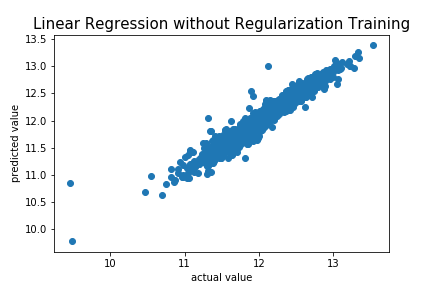
\includegraphics[width=0.4\textwidth]{Linear_Regression_without_Regularization_trn.png}
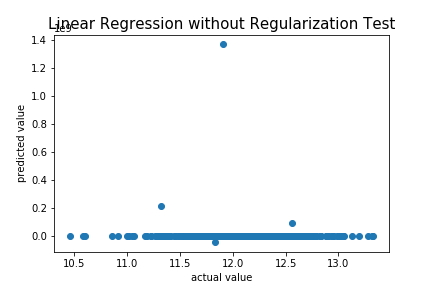
\includegraphics[width=0.4\textwidth]{Linear_Regression_without_Regularization_tst.png}
\caption{How OLS without Regularization Fails to Generalize}
\end{figure}


Regularization (either L1 or L2) will add penalty to the final loss function for weights. If the weight for basement area is very huge, say $w_{\text{basementArea}}=20000$, then this will add $\lambda 20000^2$ to the final loss.\footnote{The number is only made up. Also in the real model, I do log transformation for Sale Price and various features.} It could happen that when we decrease $w_{\text{basementArea}}$ from $20000$ to $200$, the fitting error (MSE) term is only increased by 1e-5. Then even with a very small (but not zero) regularization strength $\lambda$, the model will pick a much smaller $w_{\text{basementArea}}$ and thus makes more sense. The thing to remember: never make prediction without regularization.

\begin{figure}[H]
\centering
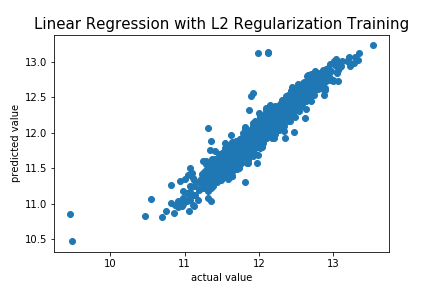
\includegraphics[width=0.4\textwidth]{Linear_Regression_with_L2_Regularization_trn.png}
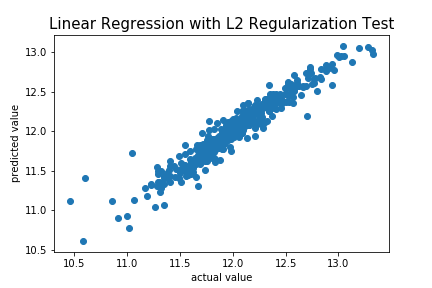
\includegraphics[width=0.4\textwidth]{Linear_Regression_with_L2_Regularization_tst.png}
\caption{Predicted Values for Linear Regression with L2 Regularization}
\end{figure}

The two graphs above shows the result of linear regression with L2 regularization. You can see how the predicted values change magically with the simple regularization term $\lambda \norm{W}_2^2$ added to the loss function. 

The predicted values for the remaining models won't look much different, so I won't plot them. From the table, we can see that SVR is the best choice for the house price prediction task, and Lasso is slightly worse. Random Forest, although fits the training set extremely well, is not a very good model, probably because it is hard for a tree-based model to capture a simple linear relationship between $x$ and $y$. If the real data is $y=2x+3$, then the decision tree is forced to split $x$ into small intervals, and then calculate the mean of $y$ within each interval.

\section{Unsupervised Learning}
So we've seen how supervised learning methods work for house price prediction. In this section, I'll introduce a completely different machine learning framework, unsupervised learning. 

In an unsupervised learning setup, we don't know the actual house prices at all, and we are not asked to predict house prices. The goals are rather ambiguous for unsupervised learning, and different approaches of unsupervised learning have different goals. In general, the goal is to explore patterns in the existing data. Here I'll introduce one specific unsupervised learning method, Principal Component Analysis.

\subsection{Principal Component Analysis}

Principal Component Analysis (PCA) \citep{shlens2014tutorial} is a technique to reduce the dimensionality of the data and at the same time still enable the dimensionality reduced data to well represent the original data. 

First this dimensionality reduction is presented as a linear transformation $P$ ($m\times r$) of the original data $X$ ($n\times m$). We denote the transformed data as $Z$ ($n\times r$), with $Z = XP$. $P$ reduces the data dimensionality from $m$ to $r$, with $r \leq m$. 

Then we choose the desired property of transformed data $Z$ to be removing feature redundancy and explaining data variance. To formalize things, we introduce the notation of covariance matrix. The covariance matrix of $Z$, $C_Z$ is defined as:
\begin{equation}
  C_Z \equiv \frac{1}{n} Z^T Z.
\end{equation}
$C_X$ is a square symmetric $r\times r$ matrix. The diagonal terms measure the variance explained by each feature, and the off-diagonal terms are the covariance between features. The desired property of $Z$ can thus be stated as: 1) $C_Z$ is diagonal, and 2) the diagonal values of $C_Z$ are the highest possible ones. We can derive the following:

\begin{align}
  C_Z &= \frac{1}{n} Z^T Z = \frac{1}{n} (XP)^T (XP) = \frac{1}{n} P^T X^T X P \\
 &= P^T (\frac{1}{n} X^T X) P = P^T C_X P
\end{align}

A theorem in linear algebra states that for a symmetric matrix $A$, we can decompose it as $A=EDE^T$ where $D$ is a diagonal matrix, and $E$ is a matrix of eigenvectors of $A$ arranged as columns. Thus we can select matrix $P$ to be a matrix where each column $P_{[:,j]}$ is an eigenvector of $C_X$, and by this selection, $P \equiv E$. We also know that for matrix $P$ consisting of orthonormal vectors, we have $P^TP = I$.

\begin{align}
  C_Z &= P^T C_X P = P^T (EDE^T)P = P^T (PDP^T) P \\
&= (P^TP) D (P^TP) = D
\end{align}

Now we have finished the derivation of PCA. The principal components of $X$ are the eigenvectors of $C_X = \frac{1}{n}X^TX$. The $j^{th}$ diagonal value of $C_Z$ is the variance of $X$ along $P_{[:, j]}$. The principal components (PC) are ordered so that the first principal component (PC1) corresponds to the normalized eigenvector of $C_X$ with the largest (absolute) eigenvalue, which means PC1 explains the most variance in the data. And if we remove the dimensionality of PC1, then the second principal component explains the most variance for the remaining data, etc.

This graph below\footnote{Taken from \url{https://en.wikipedia.org/wiki/Principal_component_analysis\#/media/File:GaussianScatterPCA.svg}} shows the first two principal components of a Gaussian random data. The first principal component is pointing the the upper left. If we project data onto this PC1, the projected data will have high variance.

\begin{figure}[H]
\centering
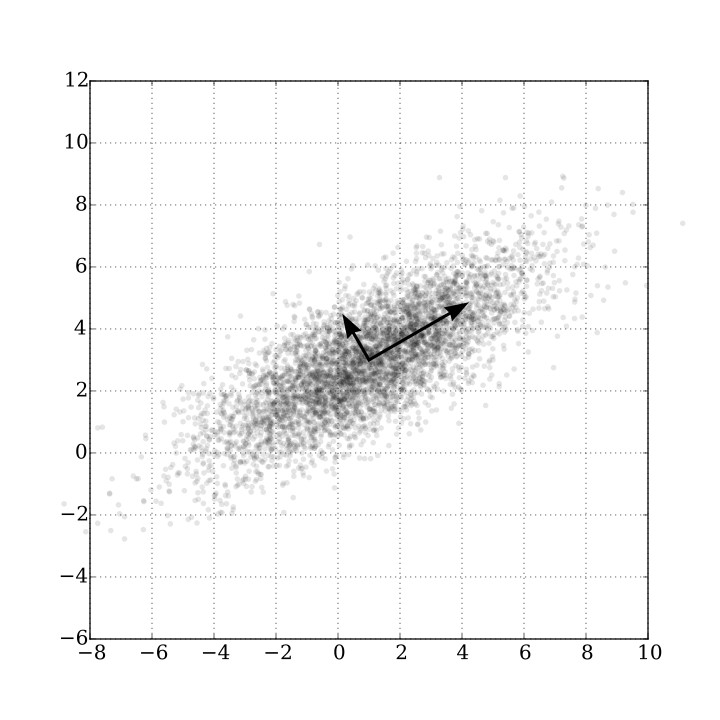
\includegraphics[width=0.6\textwidth]{GaussianScatterPCA.png}
\caption{First two Principal Components of a Gaussian Data}
\end{figure}

\subsection{Principal Component Analysis on House Features}
We've already introduced PCA. Then let's try the principal component analysis on our house features. The following analysis is conducted on the training set.

\begin{figure}[H]
\centering
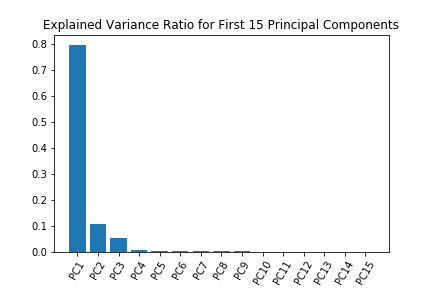
\includegraphics[width=0.7\textwidth]{pca_explained_ratio.png}
\caption{Explained Variance Ratio for First 15 Principal Components}
\end{figure}

\begin{figure}[H]
\centering
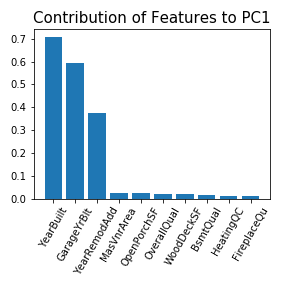
\includegraphics[width=0.3\textwidth]{contribution_to_pc1.png}
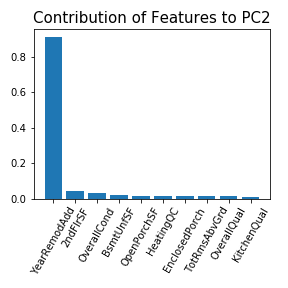
\includegraphics[width=0.3\textwidth]{contribution_to_pc2.png}
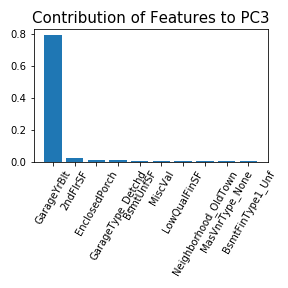
\includegraphics[width=0.3\textwidth]{contribution_to_pc3.png}
\caption{Contribution of Features to first 3 Principal Components}
\end{figure}

Although PCA is a widely adopted technique\footnote{Adopted more in classification than regression.} for extracting useful information from data, the result here doesn't really make much sense. The first three principals are mostly composed of three year related features: 1) the year the house was built, 2) the year the garage is built, 3) the year the house was most recently remodeled. 

This could be partly my bad because I forgot to do log transformation on these year variables. The variables like living area, after log transformation, won't remain much variance. Thus the untransformed year variables take on to explain most of the variance in data.

Still, the main one to blame is PCA itself. Explaining the most variance in data is really a limited standard of choosing important features. Imagine that the phone number of the house owner is accidentally included to the dataset as a continuous number variable, then phone number will probably contribute a lot to some principal component(s) because it brings a lot of variance and is not redundant at all. The computer has no idea that a phone number as a number is totally irrelevant for house price prediction. This is a problem inherent to almost all unsupervised learning methods. 

Yet on the other hand, PCA captures the patterns in the data, and the abnormal result of PCA gives us the information that probably I should also do log transformation on the year variables, or keep all variables untransformed. 

\begin{figure}[H]
\centering
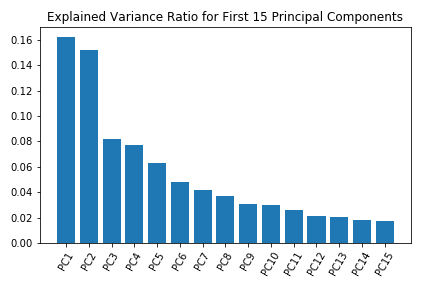
\includegraphics[width=0.7\textwidth]{pca_explained_ratio_yr.png}
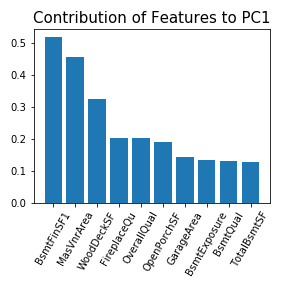
\includegraphics[width=0.3\textwidth]{contribution_to_pc1_yr.png}
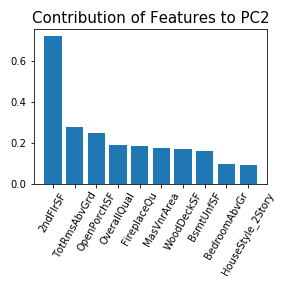
\includegraphics[width=0.3\textwidth]{contribution_to_pc2_yr.png}
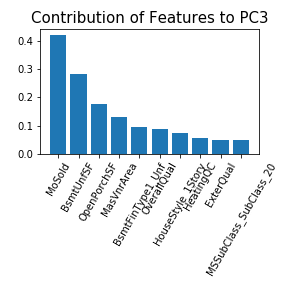
\includegraphics[width=0.3\textwidth]{contribution_to_pc3_yr.png}
\caption{Results of PCA with Year Variables also Log Transformed}
\end{figure}

Then I log transformed the three year variables and redo the PCA. The results make more sense, with explained variance distributed more evenly, and area variables taking more weight in principal components. However, I don't yet know any reliable rules of variable transformation, except for trial and error, which is only available in a supervised learning setup.\footnote{Transformation of variables belong to another huge topic in machine learning, called feature engineering. There is fewer general approaches to introduce in feature engineering, so I decide not to go into details. Here taking log for the skewed continuous variables does increase model performance. Whether to take log on the three year variables don't really affect the model prediction result.} In economics, we almost never log transform year variables, but PCA implies we should do that.

\begin{figure}[H]
\centering
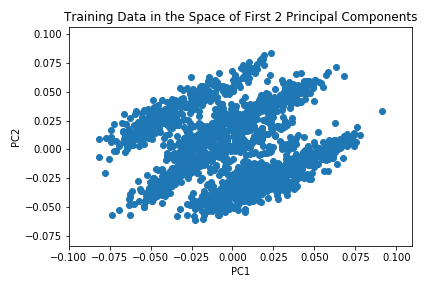
\includegraphics[width=0.7\textwidth]{data_pc_space.png}
\caption{Data in the Space of First 2 Principal Components}
\end{figure}

Here I plot the training data onto a 2D plane of the first two components. The x-axis is the first principal component, and the y-axis is the second. Something interesting seem to be going on, but I'm not going to interpret here.

So the conclusion is that PCA is easily affected by variable transformation, and thus the information from PCA is not guaranteed to make sense. Still PCA can be performed for data visualization, and perhaps useful patterns can be observed by human eyes.

\section{Feature Selection}
In the previous section, we've seen that PCA could be used to reduce the dimensionality of our data. Dimensionality reduction is useful in helping human beings to understand the patterns in data. Yet here our goal is to make predictions. Is it possible that reduced data dimensionality also helps the model to make predictions? The answer is that it depends. 

Below I'll show the model prediction results with four different set of features: 
\begin{enumerate}
  \item 5 hand picked features, GrLivArea (living area above ground), TotalBsmtSF (total sqft of basement area), LotArea (lot area), OverallCond (overall condition), and OverallQual (overall quality). 
  \item First 5 principal Components, with year variables also log transformed.
  \item 146 features selected using Lasso regression. First tune a Lasso regression model on the full feature data, then drop the features with zero weight in the Lasso predictor.
  \item First 146 principal Components, with year variables also log transformed. The number 146 is chosen to compare with the Lasso selected features.
\end{enumerate}

\begin{table}[H]
\centering
\caption{\large Results with 5 Hand Picked Features}
\vspace{0.3cm}
\begin{tabular}{| r | p{2cm} | p{2cm} | p{2cm} |}
\hline
 & \multicolumn{3}{|c|}{Results: (RMSE, $R^2$)} \\
\hline
Model & Training & Validation & Test \\
\hline
Linear Regression without Regularization (OLS) & 0.1836, 0.795 & 0.1648, 0.843 & 0.1795, 0.810 \\
\hline
Linear Regression with L2 Regularization & 0.1836, 0.795 & 0.1648, 0.843 & 0.1795, 0.810 \\
\hline
Lasso Regression & 0.1836, 0.795 & 0.1648, 0.843 & 0.1795, 0.810 \\
\hline
Support Vector Regression & 0.1629, 0.839 & 0.1451, 0.878 & 0.1644, 0.841 \\
\hline
Random Forest Regression & 0.0622, 0.977 & 0.1522, 0.866 & 0.1713, 0.827 \\
\hline
\end{tabular}
\end{table}

\begin{table}[H]
\centering
\caption{\large Results with First 5 Principal Components}
\vspace{0.3cm}
\begin{tabular}{| r | p{2cm} | p{2cm} | p{2cm} |}
\hline
 & \multicolumn{3}{|c|}{Results: (RMSE, $R^2$)} \\
\hline
Model & Training & Validation & Test \\
\hline
Linear Regression without Regularization (OLS) & 0.2346, 0.665 & 0.2230, 0.712 & 0.2391, 0.663 \\
\hline
Linear Regression with L2 Regularization & 0.2346, 0.665 & 0.2230, 0.712 & 0.2391, 0.663 \\
\hline
Lasso Regression & 0.2346, 0.665 & 0.2230, 0.712 & 0.2391, 0.663 \\
\hline
Support Vector Regression & 0.2350, 0.664 & 0.2258, 0.705 & 0.2404, 0.659 \\
\hline
Random Forest Regression & 0.0768, 0.964 & 0.1888, 0.794 & 0.2131, 0.732 \\
\hline
\end{tabular}
\end{table}


\begin{table}[H]
\centering
\caption{\large Results with 146 Lasso Features}
\vspace{0.3cm}
\begin{tabular}{| r | p{2cm} | p{2cm} | p{2cm} |}
\hline
 & \multicolumn{3}{|c|}{Results: (RMSE, $R^2$)} \\
\hline
Model & Training & Validation & Test \\
\hline
Linear Regression without Regularization (OLS) & 0.1019, 0.937 & 0.1162, 0.922 & 0.1150, 0.922 \\
\hline
Linear Regression with L2 Regularization & 0.1150, 0.920 & 0.1162, 0.922 & 0.1185, 0.917 \\
\hline
Lasso Regression\footnote{Applied again, allowing Lasso to select a smaller subset of features} & 0.1049, 0.933 & 0.1127, 0.927 & 0.1139, 0.923 \\
\hline
Support Vector Regression & 0.1184, 0.915 & 0.1064, 0.935 & 0.1164, 0.920 \\
\hline
Random Forest Regression & 0.0506, 0.984 & 0.1289, 0.904 & 0.1315, 0.898 \\
\hline
\end{tabular}
\end{table}

\begin{table}[H]
\centering
\caption{\large Results with First 146 Principal Components}
\vspace{0.3cm}
\begin{tabular}{| r | p{2cm} | p{2cm} | p{2cm} |}
\hline
 & \multicolumn{3}{|c|}{Results: (RMSE, $R^2$)} \\
\hline
Model & Training & Validation & Test \\
\hline
Linear Regression without Regularization (OLS) & 0.1152, 0.919 & 0.1218, 0.914 & 0.1209, 0.914 \\
\hline
Linear Regression with L2 Regularization & 0.1188, 0.914 & 0.1182, 0.919 & 0.1220, 0.912 \\
\hline
Lasso Regression & 0.1205, 0.912 & 0.1178, 0.920 & 0.1241, 0.909 \\
\hline
Support Vector Regression & 0.1224, 0.909 & 0.1092, 0.931 & 0.1174, 0.919 \\
\hline
Random Forest Regression & 0.0688, 0.981 & 0.1775, 0.818 & 0.1912, 0.785 \\
\hline
\end{tabular}
\end{table}

For linear regression without regularization, using a selected set of features largely solves the failed generalization problem. However, for all other models, prediction made with fewer features perform strictly worse. Because all models with regularization\footnote{In SVR and Random Forest there is also regularization, although we don't explicitly call something regularization term.} can learn which features to use, and giving these models less information will result in strictly worse performance.

Compare table 3 with table 2, table 5 with table 4, we can see that selecting features work strictly better than transforming features with PCA. Because PCA is a lossy data transformation, and it destroys our data. So don't use principal components before making house price prediction. There are many feature selection methods in the supervised learning field, and Lasso is only one of them. If we compare these four tables with table 1, we would agree that a good model doesn't require feature selection beforehand, at least for this house price prediction task.

When we compare results of the different methods within table 2, we see that non-linear models perform strictly better than linear models. Non-linearity models are able to capture more complicated relationships within data, which is an even larger advantage over linear models when the number of features is limited.

\section{Conclusion}
Here are the things to remember when making house price prediction:
\begin{enumerate}
  \item The prediction result has to be evaluated using a test dataset that is not included during the training.
  \item Always add regularization term (explicitly or implicitly) to the model. When the number of features is limited, it doesn't harm. When the number of features is huge, it saves your life.
  \item Principal component analysis is helpful for data visualization, but not for feature selection.
  \item Choose support vector regression with no feature selection.
\end{enumerate}



\bibliographystyle{chicago}
\bibliography{hedonic}

\end{document}